%
% teil1.tex -- Euler-Spirale
%
% (c) 2020 Prof Dr Andreas Müller, Hochschule Rapperswil
%
\section{Euler-Spirale
\label{fresnel:section:eulerspirale}}
\rhead{Euler-Spirale}
\begin{figure}
\centering
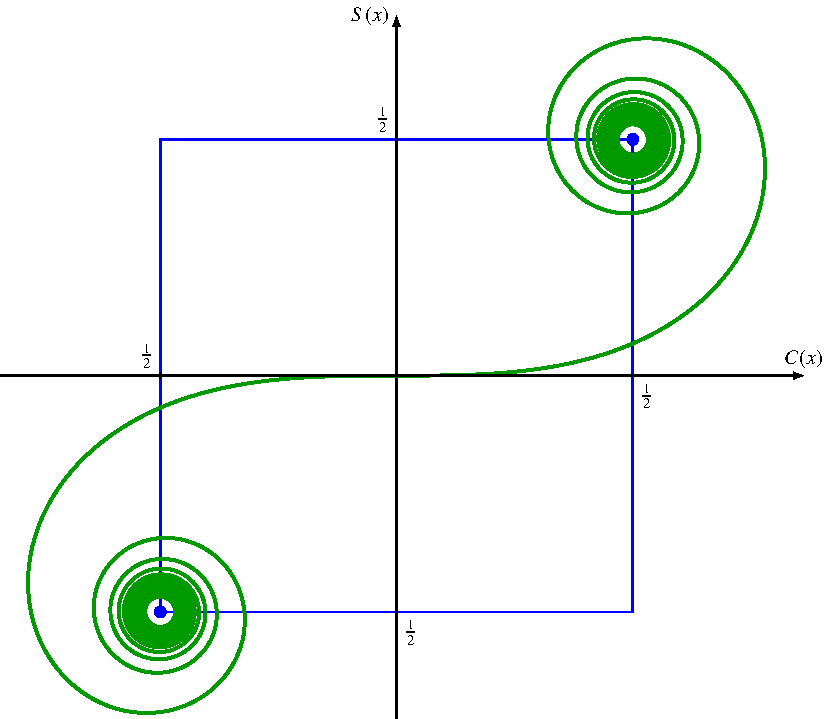
\includegraphics{papers/fresnel/images/eulerspirale.pdf}
\caption{Die Eulerspirale ist die Kurve mit der Parameterdarstellung
$x\mapsto (C(x),S(x))$, sie ist rot dargestellt.
Sie windet sich unendlich oft um die beiden Punkte $(\pm\frac12,\pm\frac12)$.
\label{fresnel:figure:eulerspirale}}
\end{figure}
Ein besseres Verständnis für die beiden Funktionen $C(x)$ und $S(x)$
als die Darstellung~\ref{fresnel:figure:plot} ermöglicht die
Abbildung~\ref{fresnel:figure:eulerspirale}, die die beiden Funktionen
als die $x$- und $y$-Koordinaten der Parameterdarstellung einer Kurve
zeigt.
Sie heisst die {\em Euler-Spirale}.
Die Spirale scheint sich für $x\to\pm\infty$ um die Punkte
$(\pm\frac12,\pm\frac12)$ zu winden.

\begin{figure}
\centering
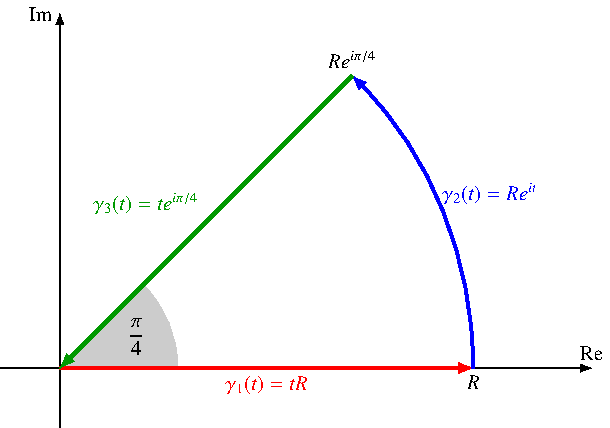
\includegraphics{papers/fresnel/images/pfad.pdf}
\caption{Pfad zur Berechnung der Grenzwerte $C_1(\infty)$ und
$S_1(\infty)$ mit Hilfe des Cauchy-Integralsatzes
\label{fresnel:figure:pfad}}
\end{figure}


\begin{satz}
Die Grenzwerte der Fresnel-Integrale für $x\to\pm\infty$ sind
\[
\lim_{x\to\pm\infty} C(x)
=
\lim_{x\to\pm\infty} S(x)
=
\frac12.
\]
\end{satz}

\begin{proof}[Beweis]
Die komplexe Funktion 
\(
f(z) = e^{-z^2}
\)
ist eine ganze Funktion, das Integral über einen geschlossenen
Pfad in der komplexen Ebene verschwindet daher.
Wir verwenden den Pfad in Abbildung~\ref{fresnel:figure:pfad}
bestehend aus den drei Segmenten $\gamma_1$ entlang der reellen
Achse von $0$ bis $R$, dem Kreisbogen $\gamma_2$ um $0$ mit Radius $R$
und $\gamma_3$ mit der Parametrisierung $t\mapsto te^{i\pi/4}$.

Das Teilintegral über $\gamma_1$ ist
\[
\lim_{R\to\infty}
\int_{\gamma_1} e^{-z^2}\,dz
=
\int_0^\infty e^{-t^2}\,dt
=
\frac{\sqrt{\pi}}2.
\]
Das Integral über $\gamma_3$ ist
\begin{align*}
\lim_{R\to\infty}
\int_{\gamma_3} 
e^{-z^2}\,dz
&=
-\int_0^\infty \exp(-t^2 e^{i\pi/2}) e^{i\pi/4}\,dt
=
-
\int_0^\infty e^{-it^2}\,dt\,
e^{i\pi/4}
\\
&=
-e^{i\pi/4}\int_0^\infty \cos t^2 - i \sin t^2\,dt
\\
&=
-\frac{1}{\sqrt{2}}(1+i)
\bigl(
C_1(\infty)
-i
S_1(\infty)
\bigr)
\\
&=
-\frac{1}{\sqrt{2}}
\bigl(
C_1(\infty)+S_1(\infty)
+
i(C_1(\infty)-S_1(\infty))
\bigr),
\end{align*}
wobei wir
\[
C_1(\infty) = \lim_{R\to\infty} C_1(R)
\qquad\text{und}\qquad
S_1(\infty) = \lim_{R\to\infty} S_1(R)
\]
abgekürzt haben.

Das Integral über das Segment $\gamma_2$ lässt sich
mit der Parametrisierung
\(
\gamma_2(t)
=
Re^{it}
=
R(\cos t + i\sin t)
\)
wie folgt
abschätzen:
\begin{align*}
\biggl|\int_{\gamma_2} e^{-z^2} \,dz\biggr|
&=
\biggl|
\int_0^{\frac{\pi}4}
\exp(-R^2(\cos 2t + i\sin 2t)) iR e^{it}\,dt
\biggr|
\\
&\le
R
\int_0^{\frac{\pi}4}
e^{-R^2\cos 2t}
\,dt
\le
R
\int_0^{\frac{\pi}4}
e^{-R^2(1-\frac{4}{\pi}t)}
\,dt.
\intertext{Dabei haben wir $\cos 2t\ge 1-\frac{4}\pi t$ verwendet.
Mit dieser Vereinfachung kann das Integral ausgewertet werden und
ergibt}
&=
Re^{-R^2}
\int_0^{\frac{\pi}4}
e^{R^2\frac{\pi}4t}
\,dt
=
Re^{-R^2}
\biggl[
\frac{4}{\pi R^2}
e^{R^2\frac{\pi}4t}
\biggr]_0^{\frac{\pi}4}
=
\frac{4}{\pi R}
e^{-R^2}(e^{R^2}-1)
=
\frac{4}{\pi R}
(1-e^{-R^2})
\to 0
\end{align*}
für $R\to \infty$.
Im Grenzwert $R\to \infty$ kann der Teil $\gamma_2$ des Pfades
vernachlässigt werden.

Das Integral über den geschlossenen Pfad $\gamma$ verschwindet.
Da der Teil $\gamma_2$ keine Rolle spielt, müssen sich die
Integrale über $\gamma_1$ und $\gamma_3$ wegheben, also
\begin{align*}
0
=
\int_\gamma e^{-z^2}\,dz
&=
\int_{\gamma_1} e^{-z^2}\,dz
+
\int_{\gamma_2} e^{-z^2}\,dz
+
\int_{\gamma_3} e^{-z^2}\,dz
\\
&\to
\frac{\sqrt{\pi}}2
-\frac{1}{\sqrt{2}}(C_1(\infty)+S_1(\infty))
-\frac{i}{\sqrt{2}}(C_1(\infty)-S_1(\infty)).
\end{align*}
Der Imaginärteil ist $C_1(\infty)-S_1(\infty)$, da er verschwinden
muss, folgt $C_1(\infty)=S_1(\infty)$.
Nach Multlikation mit $\sqrt{2}$ folgt aus der Tatsache, dass auch
der Realteil verschwinden muss
\[
\sqrt{\frac{\pi}{2}} = C_1(\infty)+S_1(\infty)
\qquad
\Rightarrow
\qquad
C_1(\infty)
=
S_1(\infty)
=
\frac12
\sqrt{
\frac{\pi}{2}
}.
\]
Aus
\eqref{fresnel:equation:arg}
erhält man dann auch die Grenzwerte
\[
C(\infty)=S(\infty)=\frac12.
\qedhere
\]
\end{proof}
